\index{differential equations}
\index{ODE}
\chapter{Differential Equations}
\newthought{Simulating Dynamic Systems Numerically}


% ==============================================================================================
% INTRODUCTION BLOCK

\section{The Why}
\index{differential equations!motivation}

\newthought{Many systems} are described not by what they are, but by how they change:
\begin{itemize}
    \item Population growth: $\frac{dP}{dt} = rP$ (rate proportional to size)
    \item Radioactive decay: $\frac{dN}{dt} = -\lambda N$
    \item Newton's laws: $F = ma = m\frac{d^2x}{dt^2}$
    \item Heat diffusion: $\frac{\partial u}{\partial t} = \alpha \nabla^2 u$
    \item Neural activity: $\tau \frac{dV}{dt} = -V + I(t)$ (leaky integrate-and-fire)
\end{itemize}

\newthought{Differential equations} express relationships between quantities and their rates of change.
They are the language of physics, biology, economics, and increasingly, machine learning.
The catch: most differential equations cannot be solved analytically. We need numerical methods.

\marginnote[-2em]{\newthought{The connection to deep learning is profound:}
\begin{itemize}
    \item ResNets $\approx$ Euler discretization of an ODE
    \item Neural ODEs treat depth as continuous
    \item Diffusion models solve SDEs
    \item RNNs are discrete dynamical systems
\end{itemize}}

\newthought{In machine learning and artificial intelligence,} differential equations appear everywhere:
\begin{itemize}
    \item \textbf{ResNets as Euler:} The residual connection $h_{l+1} = h_l + f(h_l)$ is an Euler step for $\frac{dh}{dt} = f(h)$
    \item \textbf{Neural ODEs:} Chen et al. (2018) proposed treating network depth as continuous time
    \item \textbf{Diffusion models:} DALL-E, Stable Diffusion, and Midjourney generate images by solving reverse stochastic differential equations
    \item \textbf{RNNs/LSTMs:} Discrete dynamical systems modeling temporal dependencies
    \item \textbf{Physics-informed NNs:} Learn solutions that satisfy physical laws expressed as PDEs
    \item \textbf{Normalizing flows:} Continuous normalizing flows use ODEs for density estimation
\end{itemize}

\newthought{Key insight:} Understanding ODE solvers means understanding what ResNets are actually doing, and why diffusion models can generate images so efficiently.



\newpage
\subsection{Hands On Experience}
\index{ODE!hands-on}

\newthought{Consider the simple ODE:}
\begin{equation}
    \frac{dy}{dt} = -y, \quad y(0) = 1
\end{equation}

This models exponential decay---radioactive material, cooling coffee, or forgetting curves. The exact solution is $y(t) = e^{-t}$. At $t = 1$: $y(1) = e^{-1} \approx 0.3679$.

\vspace{1em}
\textbf{Euler method} with step $h = 0.5$ (2 steps to reach $t=1$):

The idea: follow the tangent line at each point.
\begin{align*}
    y_0 &= 1 \quad \text{(initial condition)} \\
    y_1 &= y_0 + h \cdot f(t_0, y_0) = 1 + 0.5 \cdot (-1) = 0.5 \\
    y_2 &= y_1 + h \cdot f(t_1, y_1) = 0.5 + 0.5 \cdot (-0.5) = 0.25
\end{align*}

Our approximation: $y(1) \approx 0.25$. Error: $|0.3679 - 0.25| = 0.118$ (32\% error).

\marginnote{\newthought{Geometric view:} Euler's method follows the tangent line at each point. Since the curve bends, we always ``overshoot'' the true solution for this decay problem.}

\vspace{1em}
\textbf{With $h = 0.25$} (4 steps):
\begin{align*}
    y_0 &= 1 \\
    y_1 &= 1 + 0.25 \cdot (-1) = 0.75 \\
    y_2 &= 0.75 + 0.25 \cdot (-0.75) = 0.5625 \\
    y_3 &= 0.5625 + 0.25 \cdot (-0.5625) = 0.4219 \\
    y_4 &= 0.4219 + 0.25 \cdot (-0.4219) = 0.3164
\end{align*}

\marginnote{\newthought{Halving $h$} roughly halves the error. This suggests $O(h)$ convergence for Euler's method---first-order accuracy.}

Error: $|0.3679 - 0.3164| = 0.052$ (14\% error)---about half the previous error.

\vspace{1em}
\textbf{Pattern:} Halving the step size roughly halves the error. This is characteristic of a first-order method.

\begin{table*}[ht]
\centering
\begin{tabular}{p{0.15\textwidth}p{0.10\textwidth}p{0.22\textwidth}p{0.25\textwidth}}
\toprule
\textbf{Step size} $h$ & \textbf{Steps} & \textbf{Approximation} & \textbf{Error} \\
\midrule
1.0 & 1 & 0.000 & 0.368 (100\%) \\
0.5 & 2 & 0.250 & 0.118 (32\%) \\
0.25 & 4 & 0.316 & 0.052 (14\%) \\
0.125 & 8 & 0.344 & 0.024 (6.5\%) \\
0.0625 & 16 & 0.356 & 0.012 (3.3\%) \\
\bottomrule
\end{tabular}
\vspace{2em}
\caption{Euler's method convergence for $y' = -y$: halving the step size roughly halves the error, confirming first-order accuracy.}
\label{tab:euler_convergence}
\end{table*}


\vspace{2em}
\newthought{The Learning Objectives} of this chapter aim at providing you with the abilities to:
\begin{itemize}
    \item Formulate initial value problems (IVPs) and convert higher-order ODEs to systems
    \item Derive and apply Euler's method from Taylor expansion
    \item Understand and implement Runge-Kutta methods (RK2 and RK4)
    \item Analyze stability of numerical ODE solvers using the test equation
    \item Connect ODE solvers to ResNets, Neural ODEs, and diffusion models
    \item Choose appropriate methods for different problem types
\end{itemize}




% ==============================================================================================
% MAIN THEORY BLOCK

\newpage
\section{Initial Value Problems}
\index{initial value problem}

\newthought{An initial value problem} (IVP) consists of:
\begin{equation}
    \boxed{\frac{dy}{dt} = f(t, y), \quad y(t_0) = y_0}
\end{equation}

\begin{itemize}
    \item $f(t, y)$: function describing the rate of change (may depend on both time and current state)
    \item $y_0$: initial condition (where the solution starts)
    \item Goal: find $y(t)$ for $t > t_0$
\end{itemize}

\marginnote{\newthought{Existence and uniqueness:} Under mild conditions (Lipschitz continuity of $f$ in $y$), the IVP has a unique solution. This is the Picard-Lindelöf theorem.}

\newthought{The function $f(t,y)$} tells us the slope of the solution curve at any point. The ODE defines a \emph{slope field}: at every point $(t, y)$, there's an arrow pointing in direction $f(t, y)$. The solution curve must follow these arrows.

\newthought{Examples of IVPs:}

\begin{table*}[ht]
\centering
\begin{tabular}{p{0.18\textwidth}p{0.22\textwidth}p{0.18\textwidth}p{0.20\textwidth}}
\toprule
\textbf{System} & \textbf{ODE} & \textbf{Solution} & \textbf{Meaning} \\
\midrule
Exponential growth & $y' = ry$ & $y = y_0 e^{rt}$ & Rate $\propto$ current value \\
Exponential decay & $y' = -\lambda y$ & $y = y_0 e^{-\lambda t}$ & Radioactivity, cooling \\
Logistic growth & $y' = ry(1 - y/K)$ & Sigmoid curve & Growth limited by capacity \\
Harmonic oscillator & $x'' = -\omega^2 x$ & $\cos(\omega t)$ & Spring, pendulum \\
Predator-prey & $x' = \alpha x - \beta xy$ & Periodic & Population dynamics \\
\bottomrule
\end{tabular}
\vspace{2em}
\caption{Common initial value problems and their solutions. Many natural systems are described by differential equations.}
\label{tab:ivp_examples}
\end{table*}

\marginnote{\newthought{Logistic growth} models populations with limited resources. The growth rate $r$ is reduced by factor $(1-y/K)$ as population $y$ approaches carrying capacity $K$.}


\subsection{Converting Higher-Order ODEs}
\index{ODE!higher-order conversion}

\newthought{Second-order ODEs} like the harmonic oscillator $\frac{d^2x}{dt^2} = -\omega^2 x$ can be converted to first-order systems by introducing new variables.

\textbf{Example:} Harmonic oscillator $x'' = -\omega^2 x$

Let $v = \frac{dx}{dt}$ (velocity). Then:
\begin{align}
    \frac{dx}{dt} &= v \\
    \frac{dv}{dt} &= -\omega^2 x
\end{align}

\marginnote{\newthought{In vector form:}
\[
\frac{d}{dt}\begin{pmatrix} x \\ v \end{pmatrix} = \begin{pmatrix} v \\ -\omega^2 x \end{pmatrix}
\]
This is a first-order system with state vector $\mathbf{y} = (x, v)^T$.}

This is now a system of two first-order equations! In general, an $n$-th order ODE becomes a system of $n$ first-order ODEs.

\newthought{Why convert?} All our numerical methods work on first-order systems. By converting, we can solve any ODE---second-order, third-order, or systems of coupled equations.




\newpage
\section{Euler's Method}
\index{Euler method}

\newthought{The simplest ODE solver.} Euler's method approximates the derivative with a forward difference.

\subsection{Derivation from Taylor Expansion}
\index{Euler method!derivation}

From Taylor's theorem:
\begin{equation}
    y(t + h) = y(t) + h \cdot y'(t) + \frac{h^2}{2} y''(\xi)
\end{equation}
for some $\xi \in [t, t+h]$.

Since $y'(t) = f(t, y(t))$, we get:
\begin{equation}
    y(t + h) = y(t) + h \cdot f(t, y(t)) + O(h^2)
\end{equation}

Dropping the $O(h^2)$ term gives Euler's method:
\begin{equation}
    \boxed{y_{n+1} = y_n + h \cdot f(t_n, y_n)}
\end{equation}

\marginnote{\newthought{Algorithm:}
\begin{enumerate}
    \item Start with $y_0, t_0$
    \item Compute slope: $k = f(t_n, y_n)$
    \item Take step: $y_{n+1} = y_n + hk$
    \item Update time: $t_{n+1} = t_n + h$
    \item Repeat until $t_n \geq T$
\end{enumerate}}

\begin{figure}[h]
    \centering
    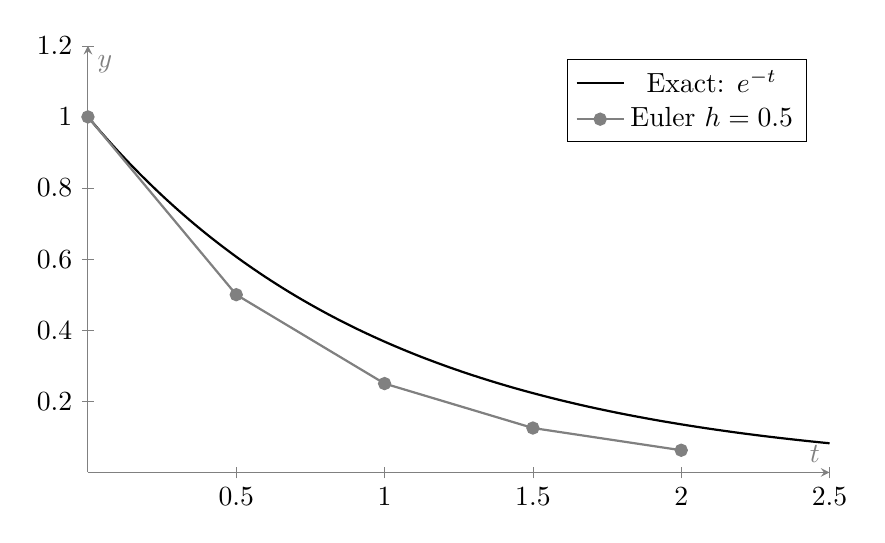
\begin{tikzpicture}
        \begin{axis}[
            width=11cm,
            height=7cm,
            axis x line=middle,
            axis y line=middle,
            xlabel={$t$},
            ylabel={$y$},
            xmin=0, xmax=2.5,
            ymin=0, ymax=1.2,
            tick style={gray},
            label style={gray},
            axis line style={gray},
            legend pos=north east,
        ]
        % Exact solution
        \addplot[black, thick, smooth, domain=0:2.5, samples=50] {exp(-x)};
        \addlegendentry{Exact: $e^{-t}$}
        % Euler steps
        \addplot[gray, thick, mark=*, mark size=2pt] coordinates {
            (0, 1) (0.5, 0.5) (1, 0.25) (1.5, 0.125) (2, 0.0625)
        };
        \addlegendentry{Euler $h=0.5$}
        % Tangent lines
        \addplot[gray, dashed, domain=0:0.5] {1 - x};
        \addplot[gray, dashed, domain=0.5:1] {0.5 - 0.5*(x-0.5)};
        \addplot[gray, dashed, domain=1:1.5] {0.25 - 0.25*(x-1)};
        \end{axis}
    \end{tikzpicture}
    \caption{Euler's method (gray) vs. exact solution (black) for $y' = -y$. Euler follows the tangent line at each step, consistently underestimating the true solution.}
    \label{fig:euler_method}
\end{figure}


\begin{algorithm}[H]
\caption{Euler's Method for ODEs}
\begin{algorithmic}[1]
    \Require Function $f(t, y)$, initial condition $y_0$, start time $t_0$, end time $T$, step size $h$
    \State $t \gets t_0$, $y \gets y_0$
    \While{$t < T$}
        \State Compute slope: $k \gets f(t, y)$
        \State Update solution: $y \gets y + h \cdot k$
        \State Update time: $t \gets t + h$
    \EndWhile
    \Return $y$
\end{algorithmic}
\end{algorithm}


\subsection{Error Analysis}
\index{Euler method!error analysis}

\newthought{Local truncation error:} The error in a single step (assuming we start exactly on the curve).
\begin{equation}
    \text{LTE} = |y(t_{n+1}) - y_{n+1}| = O(h^2)
\end{equation}

\marginnote{\newthought{Key insight:} Local error is $O(h^2)$, but we take $O(1/h)$ steps, so global error is $O(h^2) \times O(1/h) = O(h)$.}

\newthought{Global error:} The accumulated error after many steps.
\begin{equation}
    \text{Global error} = O(h)
\end{equation}

This makes Euler a \textbf{first-order method}. To get one more digit of accuracy, we need 10$\times$ more steps.


\subsection{Euler = ResNet!}
\index{ResNet}
\index{Euler method!ResNet connection}

\newthought{A profound connection:} The ResNet residual block
\begin{equation}
    h_{l+1} = h_l + f(h_l, \theta_l)
\end{equation}

is exactly one Euler step with $h = 1$ for the ODE:
\begin{equation}
    \frac{dh}{dt} = f(h(t), t)
\end{equation}

where ``time'' corresponds to layer depth.

\marginnote{\newthought{This explains:}
\begin{itemize}
    \item Why ResNets train better (smooth dynamics)
    \item Why depth helps (more accurate ODE solution)
    \item Why skip connections matter (they're the ``$+y_n$'' term!)
\end{itemize}}

This observation by Weinan E (2017) and Chen et al. (2018) launched the field of Neural ODEs.




\newpage
\section{Runge-Kutta Methods}
\index{Runge-Kutta}

\newthought{The problem with Euler:} It only samples the slope at the starting point of each step. If the slope changes significantly during the step, we accumulate error.

\newthought{Idea:} Sample the slope at multiple points within the step and take a weighted average. This gives higher-order accuracy.


\subsection{Midpoint Method (RK2)}
\index{Runge-Kutta!midpoint method}

\newthought{Sample at the midpoint:}
\begin{align}
    k_1 &= f(t_n, y_n) \quad \text{(slope at start)} \\
    k_2 &= f\left(t_n + \frac{h}{2}, y_n + \frac{h}{2} k_1\right) \quad \text{(slope at midpoint)} \\
    y_{n+1} &= y_n + h \cdot k_2
\end{align}

\marginnote{\newthought{Intuition:} Use $k_1$ to take a half-step to estimate where we'll be at the midpoint. Then use the slope at the midpoint for the full step. This gives a better ``average slope.''}

\textbf{Global error:} $O(h^2)$---one order better than Euler!

\textbf{Cost:} 2 function evaluations per step (vs.\ 1 for Euler).


\subsection{Classical RK4}
\index{RK4}

\newthought{The workhorse of ODE solving.} RK4 samples the slope at four points:

\begin{align}
    k_1 &= f(t_n, y_n) \\
    k_2 &= f\left(t_n + \frac{h}{2}, y_n + \frac{h}{2} k_1\right) \\
    k_3 &= f\left(t_n + \frac{h}{2}, y_n + \frac{h}{2} k_2\right) \\
    k_4 &= f(t_n + h, y_n + h \cdot k_3) \\
    y_{n+1} &= y_n + \frac{h}{6}(k_1 + 2k_2 + 2k_3 + k_4)
\end{align}

\marginnote{\newthought{The weights} $(1, 2, 2, 1)/6$ come from Simpson's rule! RK4 essentially integrates the slope with Simpson's quadrature.}

\newthought{Global error:} $O(h^4)$---four orders better than Euler!

\newthought{Why the weighting?} The weights $\frac{1}{6}(1 + 2 + 2 + 1) = 1$ are chosen to cancel as many Taylor series error terms as possible. This is analogous to how Simpson's rule achieves $O(h^4)$ in numerical integration.

\begin{algorithm}[H]
\caption{Classical Runge-Kutta Method (RK4)}
\begin{algorithmic}[1]
    \Require Function $f(t, y)$, initial condition $y_0$, start time $t_0$, end time $T$, step size $h$
    \State $t \gets t_0$, $y \gets y_0$
    \While{$t < T$}
        \State $k_1 \gets f(t, y)$
        \State $k_2 \gets f(t + h/2, y + h \cdot k_1/2)$
        \State $k_3 \gets f(t + h/2, y + h \cdot k_2/2)$
        \State $k_4 \gets f(t + h, y + h \cdot k_3)$
        \State Update solution: $y \gets y + \frac{h}{6}(k_1 + 2k_2 + 2k_3 + k_4)$
        \State Update time: $t \gets t + h$
    \EndWhile
    \Return $y$
\end{algorithmic}
\end{algorithm}


\subsection{Detailed Example: RK4 for Exponential Decay}
\index{RK4!example}

\newthought{Problem:} $y' = -y$, $y(0) = 1$, find $y(1)$ with a single step ($h = 1$).

\begin{align*}
    k_1 &= f(0, 1) = -1 \\
    k_2 &= f(0.5, 1 + 0.5 \cdot (-1)) = f(0.5, 0.5) = -0.5 \\
    k_3 &= f(0.5, 1 + 0.5 \cdot (-0.5)) = f(0.5, 0.75) = -0.75 \\
    k_4 &= f(1, 1 + 1 \cdot (-0.75)) = f(1, 0.25) = -0.25 \\
    y_1 &= 1 + \frac{1}{6}\bigl((-1) + 2(-0.5) + 2(-0.75) + (-0.25)\bigr) \\
    &= 1 + \frac{1}{6}(-3.75) = 1 - 0.625 = 0.375
\end{align*}

\marginnote{\newthought{Comparison:}
\begin{itemize}
    \item Exact: $e^{-1} = 0.3679$
    \item RK4: $0.375$ (1.9\% error)
    \item Euler: $0.0$ (100\% error!)
\end{itemize}
With just one step, RK4 is remarkably accurate.}

Exact: $e^{-1} = 0.3679$. Error: $|0.375 - 0.3679| = 0.007$ (1.9\%).

Compare to Euler with $h=1$: $y_1 = 1 + 1 \cdot (-1) = 0$ (100\% error!).


\subsection{Method Comparison}
\index{ODE!method comparison}

\begin{table*}[ht]
\centering
\begin{tabular}{p{0.15\textwidth}p{0.18\textwidth}p{0.10\textwidth}p{0.15\textwidth}p{0.15\textwidth}}
\toprule
\textbf{Method} & \textbf{Eval./step} & \textbf{Order} & \textbf{Error ($h=0.5$)} & \textbf{Error ($h=0.1$)} \\
\midrule
Euler & 1 & $O(h)$ & 0.118 (32\%) & 0.034 (9\%) \\
RK2 (Midpoint) & 2 & $O(h^2)$ & 0.028 (8\%) & 0.001 (0.3\%) \\
RK4 & 4 & $O(h^4)$ & 0.0007 (0.2\%) & $10^{-7}$ \\
\bottomrule
\end{tabular}
\vspace{2em}
\caption{ODE solver comparison for $y' = -y$. RK4 achieves dramatically higher accuracy for the same step size.}
\label{tab:ode_method_comparison}
\end{table*}

\marginnote{\newthought{Rule of thumb:} Use RK4 unless you have a reason not to. It's the default choice for non-stiff problems.}

\newthought{Observation:} RK4 with large $h$ often beats Euler with small $h$, even accounting for the extra function evaluations!




\newpage
\section{Stability Analysis}
\index{stability!ODE}

\newthought{Not all methods work} for all problems. A method can be accurate (small local error) but still blow up. Stability is about whether errors grow or decay.


\subsection{The Test Equation}
\index{stability!test equation}

The canonical test problem:
\begin{equation}
    \frac{dy}{dt} = \lambda y, \quad y(0) = 1
\end{equation}

where $\lambda$ is complex. For $\text{Re}(\lambda) < 0$, the exact solution $y = e^{\lambda t}$ decays.

\newthought{Euler applied to test equation:}
\begin{equation}
    y_{n+1} = y_n + h \cdot \lambda y_n = (1 + h\lambda) y_n
\end{equation}

After $n$ steps:
\begin{equation}
    y_n = (1 + h\lambda)^n y_0
\end{equation}

\marginnote{\newthought{Stability criterion:} The numerical solution stays bounded if and only if $|1 + h\lambda| \leq 1$.}

\newthought{Stability region:} The set of $z = h\lambda$ where $|1 + z| \leq 1$.

For Euler, this is a disk of radius 1 centered at $z = -1$.

\begin{figure}[h]
    \centering
    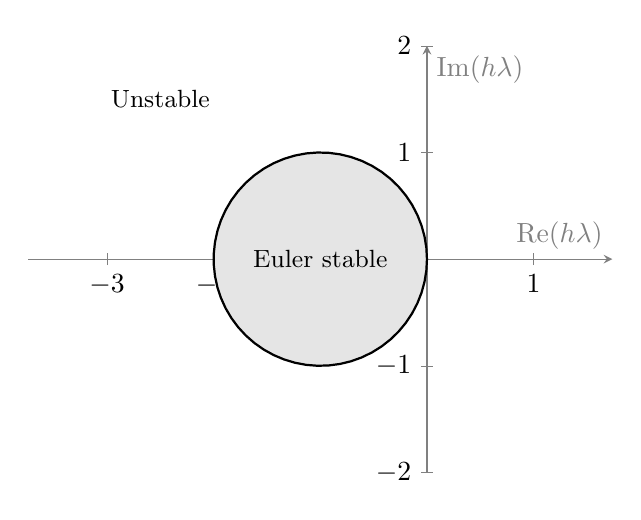
\begin{tikzpicture}
        \begin{axis}[
            width=9cm,
            height=7cm,
            axis equal,
            axis x line=middle,
            axis y line=middle,
            xlabel={Re($h\lambda$)},
            ylabel={Im($h\lambda$)},
            xmin=-3, xmax=1,
            ymin=-2, ymax=2,
            tick style={gray},
            label style={gray},
            axis line style={gray},
        ]
        % Stability region (circle centered at -1, radius 1)
        \addplot[fill=gray!20, draw=black, thick, domain=0:360, samples=60]
            ({-1 + cos(x)}, {sin(x)});
        \node at (axis cs:-1, 0) {\small Euler stable};
        \node at (axis cs:-2.5, 1.5) {\small Unstable};
        \end{axis}
    \end{tikzpicture}
    \caption{Euler stability region: values of $h\lambda$ where the method doesn't explode. For stable ODEs ($\text{Re}(\lambda) < 0$), we need $h$ small enough that $h\lambda$ falls inside this disk.}
    \label{fig:euler_stability}
\end{figure}


\subsection{What Happens Outside the Stability Region?}
\index{stability!instability example}

\newthought{Example:} $y' = -50y$, so $\lambda = -50$ (fast decay).

Stability requires $|1 + h \cdot (-50)| < 1$, which means $|1 - 50h| < 1$, giving $h < 0.04$.

With $h = 0.05$ (just outside):
\begin{align*}
    y_0 &= 1 \\
    y_1 &= (1 - 50 \cdot 0.05) \cdot 1 = -1.5 \\
    y_2 &= (1 - 2.5) \cdot (-1.5) = 2.25 \\
    y_3 &= -3.375 \\
    &\vdots \quad \text{(oscillating and exploding!)}
\end{align*}

\marginnote{\newthought{The true solution} decays smoothly toward 0, but our numerical solution oscillates wildly! This is instability---nothing to do with accuracy.}

The solution should decay to 0, but instead it oscillates with growing amplitude!


\subsection{Stiff Equations}
\index{stiff equations}

\newthought{Stiff equations} have widely varying time scales. Example:
\begin{align}
    y_1' &= -0.01 y_1 \quad \text{(slow decay)} \\
    y_2' &= -1000 y_2 \quad \text{(fast decay)}
\end{align}

For stability, Euler needs $h < 2/1000 = 0.002$ (controlled by fastest scale).
But to resolve $y_1$, we only need $h \approx 1$.

\marginnote{\newthought{Implicit methods} like Backward Euler solve $y_{n+1} = y_n + hf(t_{n+1}, y_{n+1})$, which requires solving a (possibly nonlinear) equation at each step. The payoff: stability for any step size.}

\textbf{Problem:} We take 500$\times$ more steps than necessary for accuracy, just for stability.

\textbf{Solution:} Use implicit methods (unconditionally stable) or adaptive methods.




\newpage
\section{Neural ODEs and Modern Deep Learning}
\index{Neural ODE}

\newthought{The ResNet-ODE connection} isn't just an analogy---it's the foundation of a new class of models.


\subsection{From ResNet to Neural ODE}
\index{Neural ODE!ResNet connection}

\newthought{ResNet block:}
\begin{equation}
    h_{l+1} = h_l + f(h_l, \theta_l)
\end{equation}

\newthought{As ODE:}
\begin{equation}
    \frac{dh}{dt} = f(h(t), t; \theta)
\end{equation}

where ``time'' $t$ corresponds to layer depth, and $\theta$ parameterizes the network.

\marginnote{\newthought{Neural ODE advantages:}
\begin{itemize}
    \item Continuous depth (evaluate at any $t$)
    \item Memory efficient (adjoint method)
    \item Invertible (for normalizing flows)
    \item Adaptive computation
\end{itemize}}

\newthought{Neural ODEs} (Chen et al., 2018) take this literally:
\begin{enumerate}
    \item Parameterize $f$ with a neural network
    \item Solve the ODE with adaptive solvers (Dormand-Prince, RK45)
    \item Train by backpropagating through the solver (adjoint method)
\end{enumerate}


\subsection{Adjoint Method for Training}
\index{adjoint method}

\newthought{The memory problem:} Standard backprop stores all intermediate activations. For very deep networks (= long ODE trajectories), this is expensive.

\newthought{Adjoint method:} Instead of storing forward trajectory, solve a backwards ODE for the gradients:
\begin{equation}
    \frac{d\mathbf{a}}{dt} = -\mathbf{a}^T \frac{\partial f}{\partial h}
\end{equation}

where $\mathbf{a} = \frac{\partial L}{\partial h(t)}$ is the adjoint state.

\marginnote{\newthought{Memory:} $O(1)$ in depth! This enables arbitrarily deep (continuous) networks.}

This requires only $O(1)$ memory in ``depth,'' regardless of how many ODE solver steps are taken.


\subsection{Diffusion Models}
\index{diffusion models}

\newthought{Diffusion models} like Stable Diffusion and DALL-E generate images by solving SDEs:

\textbf{Forward process:} Gradually add noise
\begin{equation}
    dx = f(x,t)\,dt + g(t)\,dW
\end{equation}

\textbf{Reverse process:} Learn to denoise
\begin{equation}
    dx = \left[f(x,t) - g(t)^2 \nabla_x \log p_t(x)\right]dt + g(t)\,d\bar{W}
\end{equation}

\marginnote{\newthought{Better ODE solvers} $\Rightarrow$ fewer neural network evaluations $\Rightarrow$ faster image generation. This is why DPM-Solver and related methods are active research areas.}

The network learns $\nabla_x \log p_t(x)$ (the ``score function''). At generation time, we solve this reverse SDE numerically.

\textbf{Sampling speed:} Original DDPM needed 1000 steps. Modern solvers (DDIM, DPM-Solver) achieve similar quality in 20-50 steps by using better ODE discretizations.


\subsection{Why This Matters}
\index{ODE!deep learning connections}

\begin{itemize}
    \item \textbf{Understanding ResNets:} Skip connections are the ``$+y_n$'' term in Euler
    \item \textbf{Better architectures:} Higher-order solvers inspire higher-order skip connections
    \item \textbf{Stability analysis:} ODE stability $\Leftrightarrow$ training stability, vanishing/exploding gradients
    \item \textbf{Faster generation:} Better solvers = fewer diffusion steps = faster inference
\end{itemize}




% ==============================================================================================
% STUDENT ACTIVATION BLOCK

\newpage
\section{Examples \& Exercises}
\index{ODE!exercises}

\marginnote{\newthought{Code} can be found at \url{https://github.com/Quillstacks/lecturecode_numericalmethods.git}.}

\newthought{Exercise 1: Euler by hand.} Solve $y' = y$, $y(0) = 1$ on $[0, 1]$ with $h = 0.25$.

\begin{enumerate}[label=(\alph*)]
    \item Compute $y_1, y_2, y_3, y_4$ using Euler's method.
    \item Compare with the exact solution $y(t) = e^t$ at $t = 1$.
    \item Calculate the relative error. How does it compare to the decay problem?
\end{enumerate}


\vspace{2em}
\newthought{Exercise 2: RK4 step-by-step.} For $y' = -2ty$, $y(0) = 1$, compute one RK4 step with $h = 0.5$.

\begin{enumerate}[label=(\alph*)]
    \item Calculate $k_1, k_2, k_3, k_4$ explicitly.
    \item Compute $y_1$.
    \item The exact solution is $y(t) = e^{-t^2}$. Compare with $y(0.5) = e^{-0.25} \approx 0.7788$.
\end{enumerate}

\marginnote{\newthought{Hint for Exercise 2:} Be careful---$f(t,y) = -2ty$ depends on both $t$ and $y$!}


\vspace{2em}
\newthought{Exercise 3: Stability analysis.} For $y' = -100y$:
\begin{enumerate}[label=(\alph*)]
    \item What is the exact stability condition for Euler? (Find the critical $h$.)
    \item Compute 5 Euler steps with $h = 0.03$ starting from $y_0 = 1$.
    \item Repeat with $h = 0.01$. What changes?
    \item Why do stiff equations need small step sizes or implicit methods?
\end{enumerate}


\vspace{2em}
\newthought{Exercise 4: ResNet connection.} Consider a 10-layer ResNet: $h_{l+1} = h_l + f_l(h_l)$.

\begin{enumerate}[label=(\alph*)]
    \item Write this as an ODE (what is the continuous limit?).
    \item What ODE solver is the ResNet implicitly using?
    \item What would RK4-inspired residual connections look like?
    \item Why might ``continuous depth'' be useful for some applications?
\end{enumerate}


\vspace{2em}
\newthought{Exercise 5: Pendulum simulation.} The nonlinear pendulum: $\frac{d^2\theta}{dt^2} = -\sin\theta$.

\begin{enumerate}[label=(\alph*)]
    \item Convert to a first-order system (introduce $\omega = d\theta/dt$).
    \item Implement both Euler and RK4.
    \item Track total energy: $E = \frac{1}{2}\omega^2 - \cos\theta$.
    \item Which method conserves energy better? Why?
\end{enumerate}


\vspace{2em}
\newthought{Exercise 6: Order verification.} For $y' = -y$, $y(0) = 1$:
\begin{enumerate}[label=(\alph*)]
    \item Compute $y(1)$ with Euler using $h = 0.1, 0.05, 0.025, 0.0125$.
    \item Plot error vs.\ $h$ on a log-log scale.
    \item Verify the slope is approximately 1 (confirming $O(h)$ convergence).
    \item Repeat for RK4 and verify slope $\approx 4$.
\end{enumerate}




\newpage
\section{Self-Reflection and Recap}
\index{ODE!recap}

\newthought{Self-Reflection} Questions to guide your understanding:
\begin{itemize}
    \item Why is ResNet's skip connection \emph{exactly} an Euler step, not just ``similar to'' one?
    \item Why do diffusion models care about ODE solver quality? (Think: inference speed)
    \item What happens to accuracy if we make $h$ too small? (Hint: rounding errors accumulate)
    \item Could we make ``continuous depth'' networks with infinite layers? What would that mean?
    \item How does stability relate to exploding/vanishing gradients in deep networks?
    \item When would you choose Euler over RK4? (Think: cost vs.\ accuracy trade-offs)
\end{itemize}


\newthought{Recap} of Key Concepts:
\begin{itemize}
    \item \textbf{Initial value problems:} $y' = f(t,y)$, $y(t_0) = y_0$. Higher-order ODEs convert to systems.
    \item \textbf{Euler's method:} $y_{n+1} = y_n + hf(t_n, y_n)$, global error $O(h)$. Simple but low accuracy.
    \item \textbf{Runge-Kutta:} Sample slope at multiple points. RK4 has global error $O(h^4)$---the workhorse method.
    \item \textbf{Stability:} Step size must respect stability region. Test equation $y' = \lambda y$ reveals limits.
    \item \textbf{Stiff equations:} Multiple time scales force tiny steps. Use implicit methods.
    \item \textbf{ResNet = Euler:} Deep learning and numerical analysis share deep connections.
    \item \textbf{Neural ODEs:} Continuous-depth networks, memory-efficient training via adjoints.
    \item \textbf{Diffusion models:} Generate images by solving reverse SDEs---better solvers = faster generation.
\end{itemize}


\marginnote[2em]{\newthought{Teaser.} We've studied Newton's method, gradient descent, and many numerical techniques. But computing the full gradient over millions of training samples is \textbf{way too expensive}. Can we \textbf{approximate it with random samples}?}

\newthought{From exact to stochastic.} All the optimization methods we've studied compute exact gradients. But for ImageNet with 1.2 million images, each gradient step costs seconds of computation. Training requires tens of thousands of steps.

The next chapter introduces \emph{stochastic gradient descent}---the engine of modern deep learning. By approximating gradients with random mini-batches, SGD makes training feasible and, surprisingly, often finds better solutions than exact methods.



%%%%%%%%%%%%%%%%%%%%%%%%%%%%%%%%%%%%%%%%%%%%%%%%%%%%%%%%%%%%%%%%%%%%%%%%%%%%%%
